\documentclass[aspectratio=169]{beamer}
\usepackage[english]{babel}
\usepackage{booktabs,listings}
\usepackage[T1]{fontenc}
\usepackage[utf8]{inputenc}
\usepackage{dirtytalk}
\usepackage{amsmath, bm}
\usepackage{booktabs}
\usepackage{colortbl}
\newcommand{\bs}[1]{\boldsymbol{#1}}
\newcommand{\mbf}[1]{\mathbf{#1}}
\newcommand{\mrm}[1]{\mathrm{#1}}
\newcommand{\ttt}[1]{\texttt{#1}}
\lstset{basicstyle=\ttfamily}
\setlength{\parskip}{.5\baselineskip}
\usetheme[slogan=english, style=plain,mathfont=serif]{NTNU}

\definecolor{lgrey}{rgb}{0.8,0.8,0.8}
\definecolor{lgreen}{rgb}{0.6, 1, 0.6}
%
% Edit your meta data here
%
	\title{Probabilistic Tabular Diffusion for Explainable AI}
	%\subtitle{Description of my Thesis}
	%\author{Alexander J Ohrt}
    \author{Alexander J Ohrt\\[1ex]  {\small Supervisor: Kjersti Aas}}
        
	\date{04 May}

\begin{document}
    \maketitle

    % \begin{frame}[fragile]{Overview}
    % \only<1>{
    % \begin{columns}
    % \begin{column}{0.37\textwidth}
    % \begin{itemize}
    %     \item Explainable AI (XAI)
    %     \item Counterfactual Explanations (CEs)
    %     \item Generative Modelling
    %     \item Diffusion Models
    %     \item Selected Results from Thesis Work
    % \end{itemize}
    % \end{column}
    % \begin{column}[0.7\textwidth]
    %     \begin{figure}[h]
    %     \centering
    %     \includegraphics[width=0.9\linewidth]{beamerthementnu-master/figures/interpAccuracy.png}
    %     \caption{Qualitative illustration of the tradeoff between accuracy and interpretability in a set of common ML models.}
    %     \label{Fig:InterpretabilityVsAccuracy}
    %     \end{figure}
    % \end{column}
    % \end{columns}
    % }
    % \end{frame}

    \begin{frame}[fragile]{Overview}

    \only<1>{
        \begin{columns}
        \begin{column}{0.37\textwidth}
            \begin{itemize}
                \item Explainable AI (XAI)
                \item Counterfactual Explanations (CEs)
                \item Generative Modelling
                \item Diffusion Models
                \item Selected Results from Thesis Work
            \end{itemize}
        \end{column}
        \begin{column}{0.7\textwidth}
            \begin{figure}[h]
            \centering
            \includegraphics[width=0.9\linewidth]{figures/interpAccuracy.png}
            \caption{Qualitative illustration of the tradeoff between accuracy and interpretability in a set of common ML models.}
            \label{Fig:InterpretabilityVsAccuracy}
            \end{figure}
        \end{column}
        \end{columns}
    } 
    \end{frame}
    
    
    \begin{frame}[fragile]{XAI — Why?}

    \only<1>{
        \begin{columns}
        \begin{column}{0.37\textwidth}
            \begin{itemize}
                \item Open the black box
                \item Understand reasoning
                \item Debug systems
                \item Reduce risk
                \item Guarantee positive effects
                \item Legislative Reasons, e.g. GDPR, AI Act
            \end{itemize}
        \end{column}
        \begin{column}{0.7\textwidth}
            \begin{figure}
            \centering
            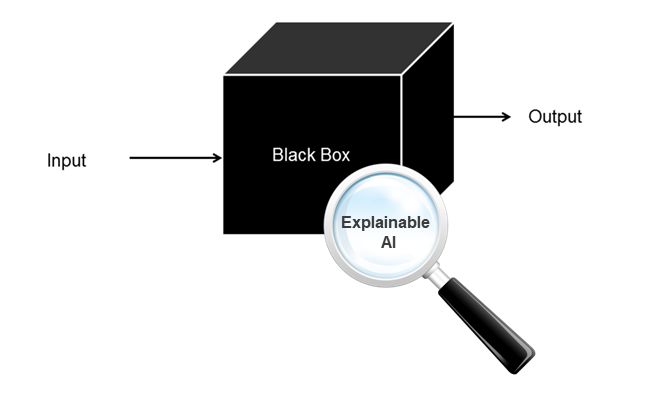
\includegraphics[width=0.99\linewidth]{figures/blackBox.png}
            \label{fig:blacBox}
            \end{figure}
        \end{column}
        \end{columns}
    } 
    \end{frame}

    \begin{frame}[fragile]{XAI — How?}

        \only<1>{
        \begin{columns}
        \begin{column}{0.37\textwidth}
            "Meta-Models": Build AI/ML models to explain other black box AI/ML models (post-hoc).
        \end{column}
        \begin{column}{0.7\textwidth}
            \begin{figure}[h]
            \centering
            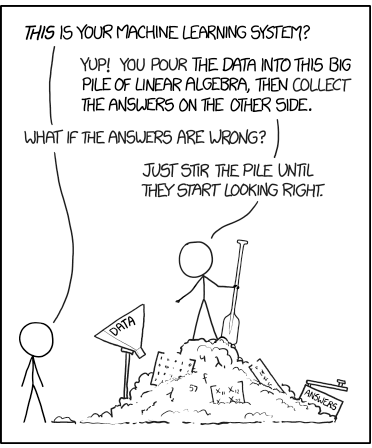
\includegraphics[width=0.55\linewidth]{figures/MLsystemMeme.png}
            \caption{Comic borrowed from \url{https://xkcd.com/1838/}}
            \label{Fig:MLsystemMeme}
            \end{figure}
        \end{column}
        \end{columns}
        }
    \end{frame}

    \begin{frame}[fragile]{XAI – How?}
        \only<1>{
            Examples of Methods:
            \begin{itemize}
                \item Shapley Values and SHAP
                \item LIME
                \item Counterfactual Explanations (CEs) 
            \end{itemize}
        }
    
    \end{frame}

    \begin{frame}[fragile]{CEs — Example}
        \begin{figure}
            \centering
            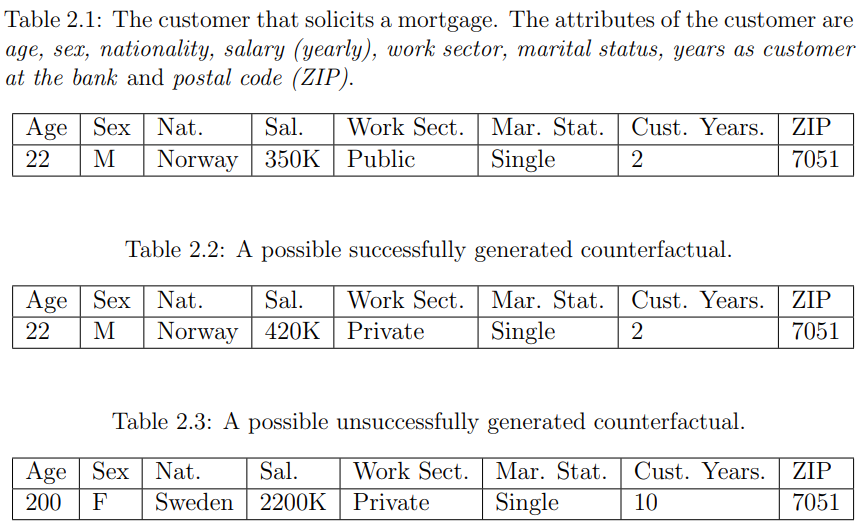
\includegraphics[scale = 0.39]{figures/counterfact_example.png}
            \label{fig:counterfactualExample}
        \end{figure}
    \end{frame}

    \begin{frame}{CEs — General Criteria}
        \begin{enumerate}
            \item \textit{on-manifold}: The counterfactual should lie on the data-manifold ("resemble the training data").
            \item \textit{actionable}: The counterfactual should not change fixed features ("not very informative to change \textit{age} e.g.").
            \item \textit{valid}: The counterfactual should flip the prediction ("from mortgage denied to mortgage granted").
            \item \textit{low cost}: The counterfactual should be as similar as possible to input ("don't change unnecessary characteristics of client").
        \end{enumerate}
    \end{frame} 

    \begin{frame}[fragile]{CEs — Algorithms}
        \onslide<1->{
            \begin{itemize}
                \item Optimization-based
            \end{itemize}
            \begin{equation}
                \min_{\bm{x}'}\{d_1(f(\bm{x}'), y') + \lambda d_2(\bm{x}, \bm{x}')\}
            \end{equation}
            \begin{itemize}
                \item On-Manifold
            \end{itemize}
        }
     
    \end{frame}

    \begin{frame}[fragile]{MCCE — Our Inspiration for Calculating CEs}
        \only<1>{
            \vspace{2em}
            MCCE: \textbf{M}onte \textbf{C}arlo sampling of realistic \textbf{C}ounterfactual \textbf{E}xplanations 
            \vspace{10em}
            \vfill
            Redelmeier, A., Jullum, M., Aas, K., \& Løland, A. (2021). MCCE: Monte Carlo sampling of realistic counterfactual explanations. arXiv preprint arXiv:2111.09790.
        }
    \end{frame}

    \begin{frame}[fragile]{MCCE — Our Inspiration for Calculating CEs}
        \onslide<1-2>{
            Steps:
            \begin{enumerate}
                \item \alt<1>{Model underlying data distribution}{\textbf{Model underlying data distribution}}
                \item \alt<1>{Sample from data distribution}{\textbf{Sample from data distribution}}
                \item Post-process the samples, i.e. filter out counterfactuals
            \end{enumerate}
        }
    \end{frame}

    \begin{frame}[fragile]{Generative Modelling with Diffusion Models}
        \begin{figure}[h]
        \centering
        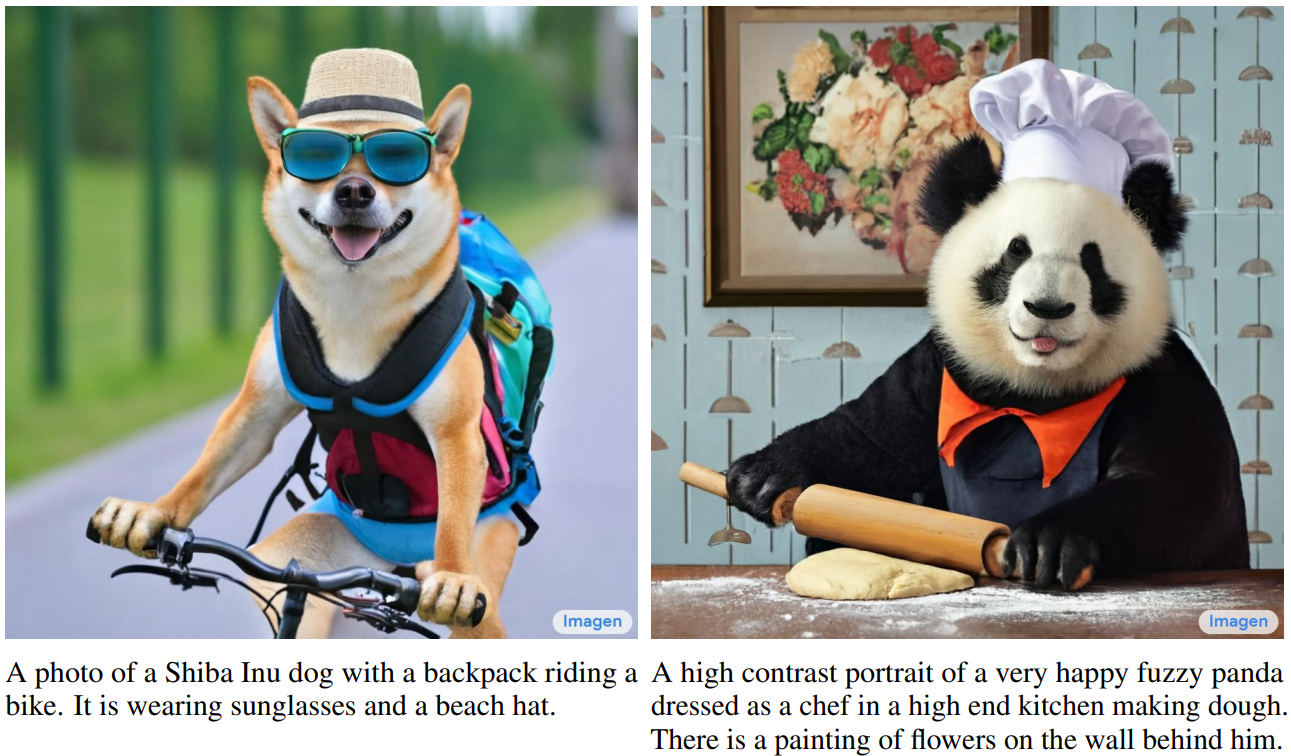
\includegraphics[width=0.68\linewidth]{figures/imagenExamples2.png}
        \caption{Examples of photorealistic images created with Imagen. Borrowed from Imagen paper (May 2022).}
        \label{Fig:ImagenExamples}
        \end{figure}
    \end{frame}

    \begin{frame}[fragile]{Diffusion Models — How?}
        \only<1>{
        \begin{figure}[h]
        \centering
        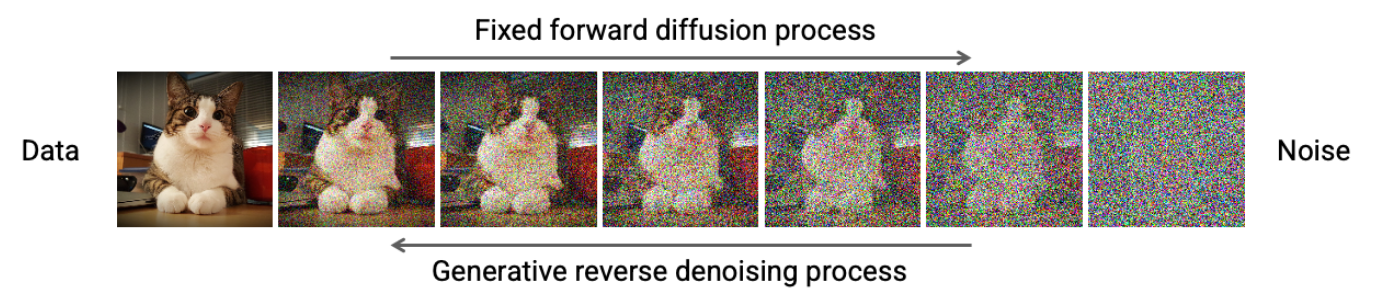
\includegraphics[width=0.9\linewidth]{figures/diffProcessIllustration.png}
        \label{Fig:DiffIllustration}
        \end{figure}
        }    
    \end{frame}

    \begin{frame}[fragile]{Diffusion Models — How?}
        \only<1>{
            \begin{figure}[h]
            \centering
            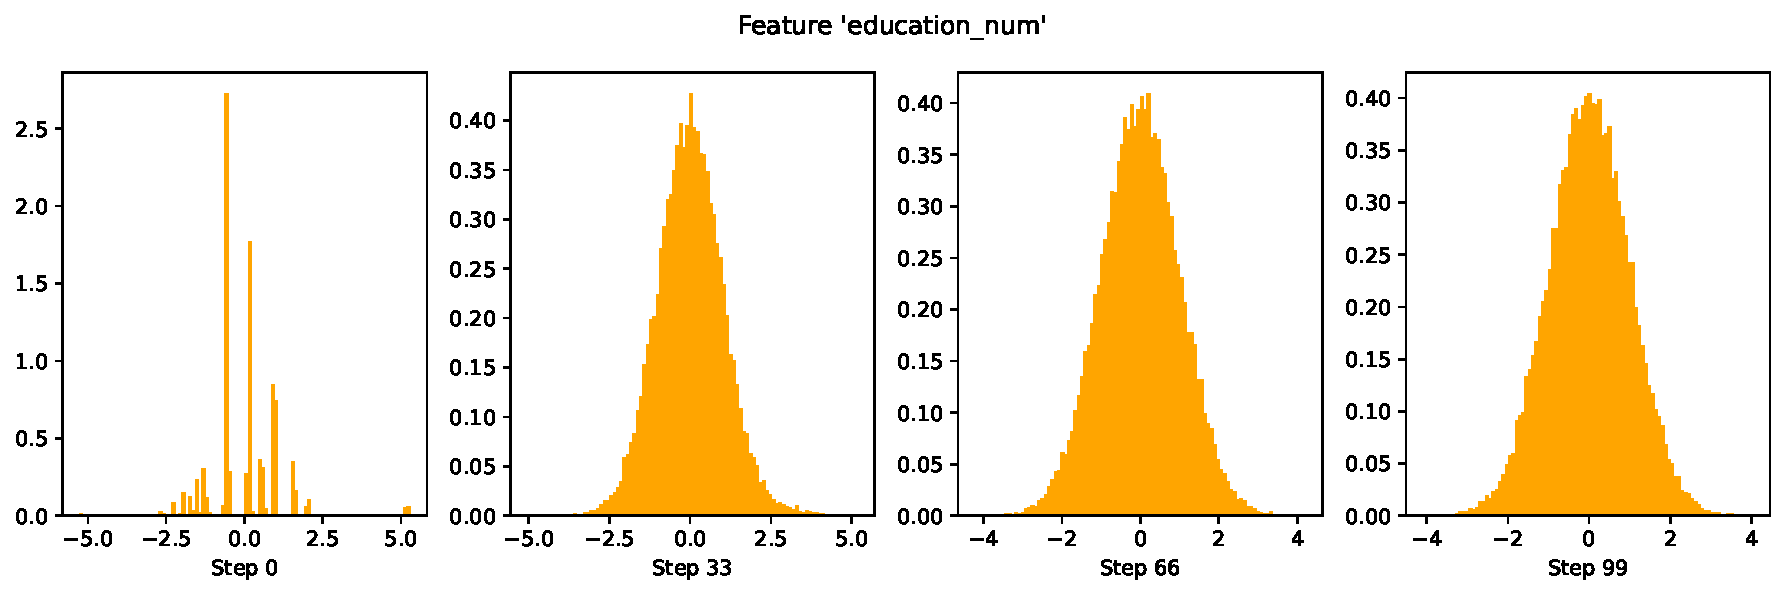
\includegraphics[width=0.99\linewidth]{figures/gaussianForwardProcess.pdf}
            \label{Fig:GaussForwardIllustration}
            \end{figure}
        }
    \end{frame}


    \begin{frame}[fragile]{Diffusion Models — How?}
        \only<1>{
            \begin{figure}[h]
            \centering
            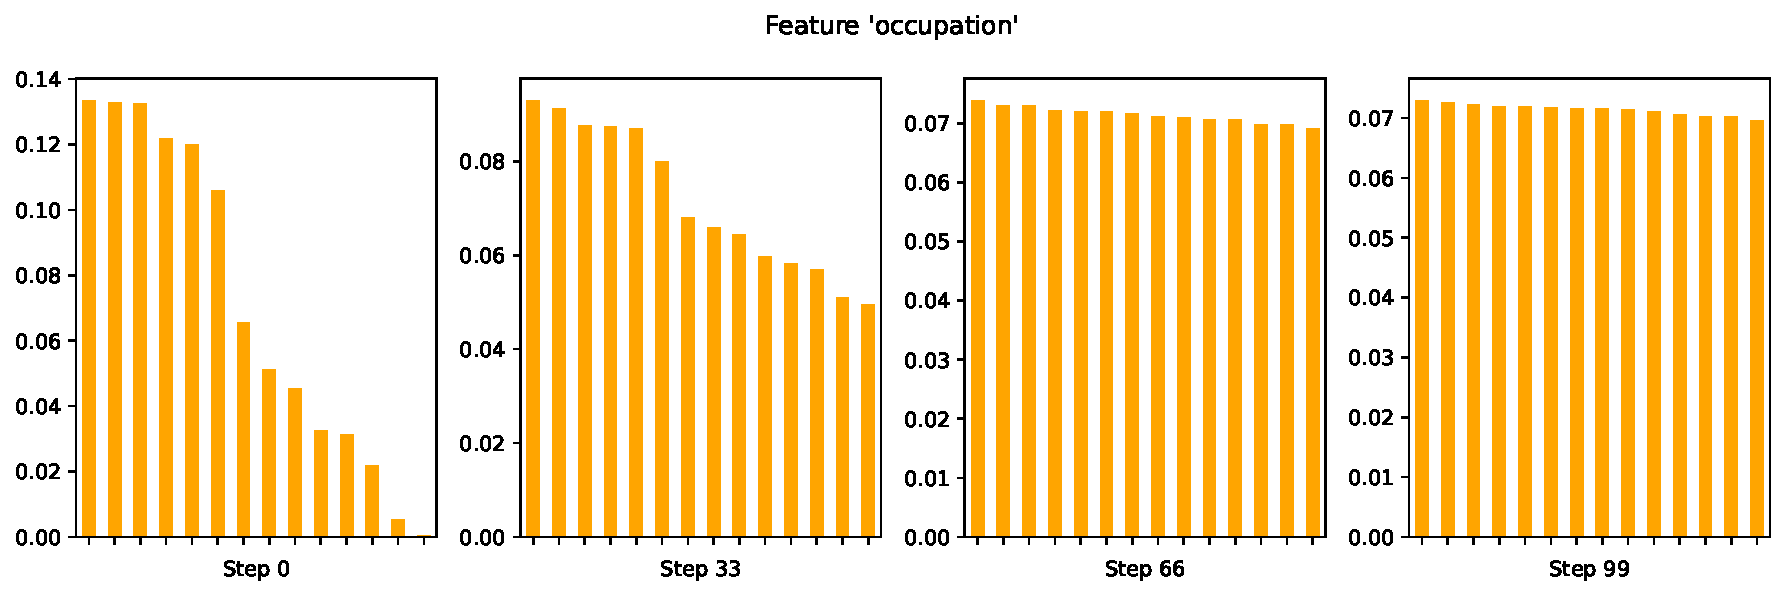
\includegraphics[width=0.99\linewidth]{figures/multinomialForwardProcess.pdf}
            \label{Fig:MultForwardIllustration}
            \end{figure}
        }
    \end{frame}

    \begin{frame}[fragile]{Thesis Objectives}
        \begin{itemize}
            \item Develop an accessible introduction to diffusion models.
            \item Implement a model specifically for \textit{tabular data}.
            \item Perform experiments. 
        \end{itemize}
    \end{frame}

    \begin{frame}[fragile]{Some Results}
        \only<1>{
        \begin{figure}[h]
            \centering
            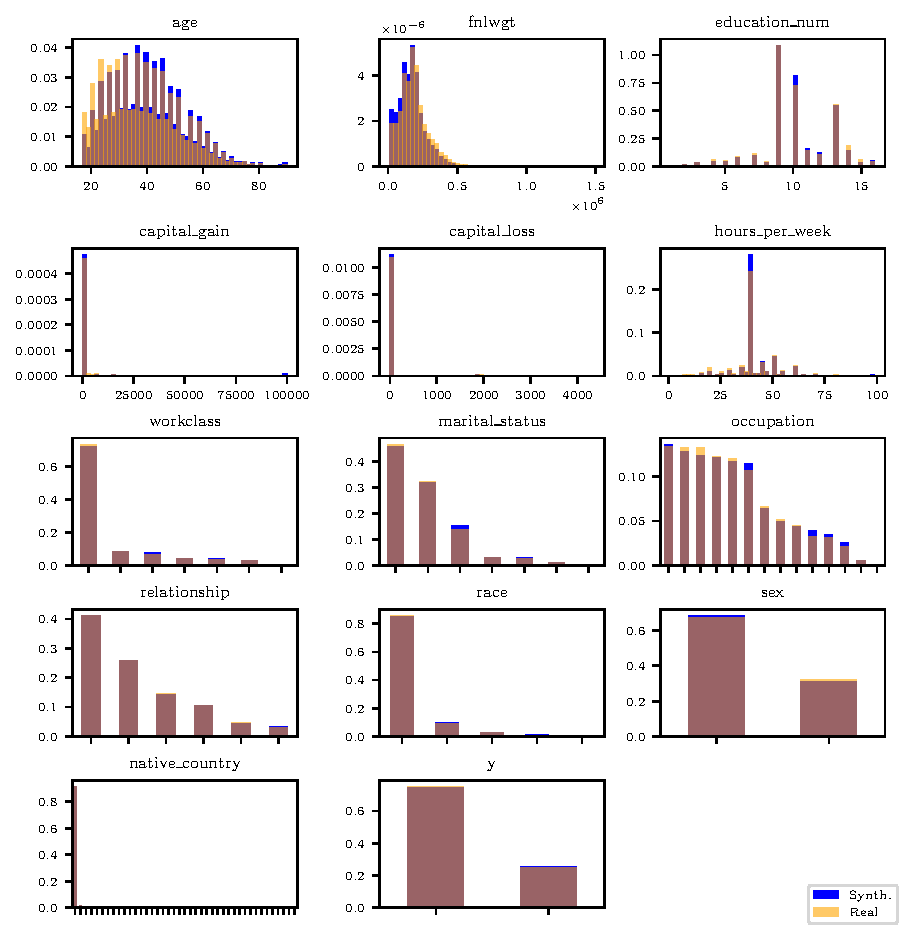
\includegraphics[width=0.5\linewidth]{figures/TabDDPM_Qual_AD_joint.pdf}
            %\caption{Marginal distributions of real and fake data.}
            \label{Fig:MarginalTabularDiffusion}
        \end{figure}
        }
        % \begin{columns}
        % \begin{column}{0.37\textwidth}
        %     \begin{figure}[h]
        %     \centering
        %     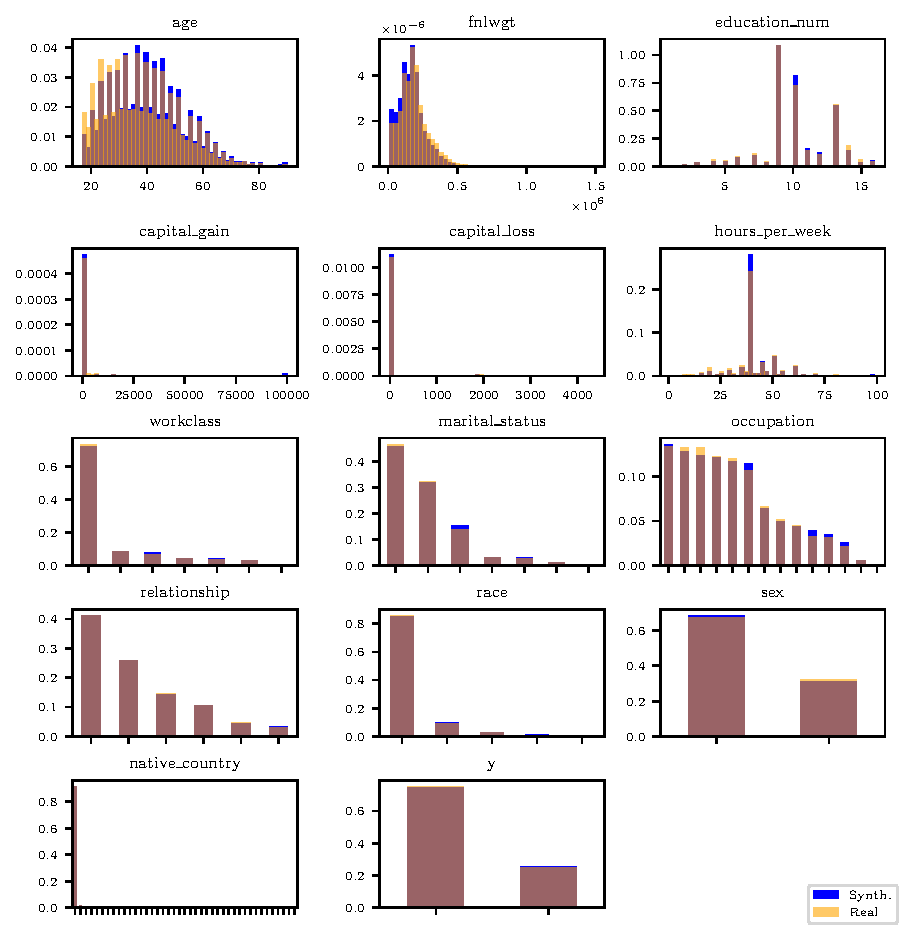
\includegraphics[width=0.5\linewidth]{figures/TabDDPM_Qual_AD_joint.pdf}
        %     \caption{Marginal distributions of real and fake data.}
        %     \label{Fig:MarginalTabularDiffusion}
        %     \end{figure}
        % \end{column}
        % \begin{column}{0.7\textwidth}
        % \begin{table}
        % \centering
        % \caption{Factual and generated counterfactual.}
        % \begin{tabular}{lll}
        % \toprule
        % {} &               $h$ &              Diffusion      \\
        % \midrule
        % \ttfamily{age}              &                25 &                   25            \\
        % \ttfamily{fnlwgt}           &            188767 &               218210             \\
        % \ttfamily{ed\_num}   &                12 &                   13                     \\
        % \ttfamily{cap\_gain}    &                 0 &                    0                 \\
        % \ttfamily{cap\_loss}    &                 0 &                 1933                  \\
        % \ttfamily{h\_p\_w} &                45 &                   52                      \\
        % \ttfamily{workcl.}        &           Private &              Private              \\
        % \ttfamily{mar\_stat}  &     Never-married &   Married   \\
        % \ttfamily{occup.}       &   Exec. &                Sales        \\
        % \ttfamily{rel.}     &     Not-family &              Husband         \\
        % \ttfamily{race}             &             White &                White            \\
        % \ttfamily{sex}              &              Male &                 Male              \\
        % \ttfamily{country}  &     US &        US         \\
        % \ttfamily{Prediction} & 0 & 1\\
        % \bottomrule
        % \end{tabular}
        % \end{table}
        % \end{column}
        % \end{columns}
    \end{frame}

    \begin{frame}[fragile]{Some Results}
        \only<1>{
        \begin{table}
        \centering
        \caption{Factual $h$ and generated counterfactual for CatBoost classifier.}
        \resizebox*{!}{0.8\textheight}{
        \begin{tabular}{lll}
        \toprule
        {} &               $h$ &              Diffusion      \\
        \midrule
        \cellcolor{lgrey}{\ttfamily{age}} & \cellcolor{lgrey}{25} & \cellcolor{lgrey}{25} \\
        \ttfamily{fnlwgt} & 188767 & \cellcolor{lgreen}{218210} \\
        \ttfamily{ed\_num}   &  12 & \cellcolor{lgreen}{13} \\
        \ttfamily{cap\_gain}    & 0 &  0  \\
        \ttfamily{cap\_loss}    & 0 & 0\\
        \ttfamily{h\_p\_w} &   45 &  \cellcolor{lgreen}{52} \\
        \ttfamily{workcl.}   &  Private & Private \\
        \ttfamily{mar\_stat}  &     Never-married &   \cellcolor{lgreen}{Married}   \\
        \ttfamily{occup.}       &   Exec. & Exec. \\
        \ttfamily{rel.}     &     Not-family &  Not-family\\
        \ttfamily{race}    & White & White \\
        \cellcolor{lgrey}{\ttfamily{sex}} & \cellcolor{lgrey}{Male} &  \cellcolor{lgrey}{Male} \\
        \ttfamily{country}  &  US &  US  \\
        \ttfamily{Prediction} & 0 & 1\\
        \bottomrule
        \end{tabular}
        }
        \end{table}
        }
    \end{frame}
\end{document}
